%---------------------------------------------------------------
\chapter{Our results}
%---------------------------------------------------------------

\todo{chapter intro}


%---------------------------------------------------------------
\section{Proofs revision}\label{sec:proofRevs}

Waniek et al. \cite{Waniek2017} proposed three hardness results for the \HL problem given degree, closeness and betweenness
centralities. In this section, we review the first two aforementioned results with respect to our definition of \HLshort.
The following text is a direct citation of the original proofs from Waniek et al.
with actual proof differences marked as bold text and notation-only differences in square brackets.

% Theorem - degree
\begin{theorem}
    The \HL problem is NP-complete given the degree centrality.
\end{theorem}
\begin{proof}
    \itshape{``
    \todo{change} The problem is trivially in NP, since after the addition of a given [|W|] it is possible to
    compute the degree centrality for all nodes in polynomial time.
    
    Next, we prove that the problem is NP-hard. To this end, we propose a reduction from the NP-complete problem of Finding k-clique.
    The decision version of this problem is defined by a network,
    $G = (V , E)$, and a constant, $k \in \mathbb{N}$, where the goal is to determine whether there exist $k$ nodes in $G$ that form a clique.
    
    Let us assume that $k \geq 3$ (if $k = 2$ then the problem is trivial). Given an instance of the problem
    of Finding k-clique, defined by some $k \geq 3$ and a network $G = (V , E)$, let us construct a network,
    $H = (V', E')$, as follows:
    
    \begin{description}
        \item[The set of nodes:] For every node, $v_i \in V$, we create a single node, $v_i$ , as well as $|N_G(v_i)|$
        other nodes, denoted by $X = \{x_{i,1},\dots, x{i,|N_G(v_i)|} \}$. Additionally, we create one node called $y$,
        as well as $\boldsymbol{n + k}$ other nodes, namely, $L' = l_1,\dots, \boldsymbol{l_{n+k}}$;
        \item[The set of edges:] We create an edge between two nodes $v_i, v_k \in V$ if and only if this edge
        was not present in $G$, i.e., $(v_i, v_j ) \in E' \Leftrightarrow (v_i, v_j ) \notin E$.
        Additionally, for every $v_i$ , we create an edge $(v_i , y)$ as well as an edge $(v_i, x_i, j)$ for every $x_i, j$.
        We also create an edge $(l_i, l_j)$ between every pair of nodes $l_i, l_j \in L'$, except for the edge $(l_1, l_2)$.
        Finally, we create two additional edges, $(l_1, y)$ and $(l_2, y)$.
    \end{description}

    An example of such an $H$ network is illustrated in [figure ommited]. Now, consider the following instance
    of the problem of hiding leaders, $(H, L, b, c, [d] )$, where:

    \begin{description}
        \item $H = (V', E')$ is the network we just constructed;
        \item $L = V' \setminus V$;
        \item $b = \frac{k\cdot(k-1)}{2}$;
        \item $c$ is the degree centrality measure;
        \item $[d] = k$. 
    \end{description}

    Next, we reduce the problem of Finding k-cliques in $G$ to the aforementioned instance of Hiding
    Leaders in $H$ . To this end, from the definition of the problem of Hiding Leaders, we know that the
    edges to be added to $H$ must be chosen from $F \times F$. Since in our instance we have:
    $F = V' \setminus L = V' \setminus (V' \setminus V ) = V$, then the edges to be added to $H$ must be chosen
    from $V \times V$ . However, since the edges in $(V \times V ) \setminus E$ are already present in $H$
    (see how $H$ is created), then the edges to be added to $H$ must be chosen from $E$.
    Out of those edges, we need to choose a subset, $[W] \subseteq E$, as a solution to the problem.
    In what follows, we will show that a solution to the above instance of the problem of \HL in $H$ corresponds
    to a solution to the problem of Finding k-clique in $G$.

    First, note that each of the k nodes with the highest degree centrality in $H$ must be a member of
    $L'$. This is because there are more than k nodes in $L'$, each of which has a degree of $\boldsymbol{n+k-1}$, while
    the degree of every node in $V' \setminus L'$ is smaller than $\boldsymbol{n + k - 1}$. Thus, for $[W]$
    to be a solution to the problem of hiding leaders, the addition of $[W]$ to $H$ must increase
    the degree of at least $k$ nodes in $V$ such that each of them has a degree of at least $n + k - 1$
    (note that the addition of $[W]$ only increases the degrees of nodes in $V$, as we already established
    that $[W] \subseteq E$). Now, since in $H$ the degree of every node in $V$ equals $n$
    (because of the way $H$ is created), then to increase the degree of $k$ such nodes to $n + k - 1$, each of them
    must be an end of at least $k - 1$ edges in $[W]$. But, since the budget in our problem instance is
    $\frac{k\cdot(k-1)}{2}$, then the only possible choice of $[W]$ is the one that increases the
    degree of exactly $k$ nodes in $V$ by exactly $k - 1$. If such a choice of $[W]$ is available, then surely
    those $k$ nodes would form a clique in $G$, since all $\frac{k\cdot(k-1)}{2}$ edges in $[W]$ are taken from $G$.
    }''
\end{proof}


% Proof
\begin{proof}\label{proofDB}
    To proof this theorem, we propose a parameterized reduction from the $k$-\textsc{Clique} problem on regular graphs,
    which is known to be W[1]-hard with respect to $k$
    
    Suppose we have a parameterized $k$-\textsc{Clique} instance $(G, k)$, where $|V(G)|=n$, $G$ is a $r$-regular graph and $n-2 \geq r \geq k \geq 3$
    (for $r > n-2$ or $r < k$ or $k < 3$ the problem is trivial).
    Then, we construct a graph $H$ in the following way:
    \begin{enumerate}
        \item Start with an empty graph $H$.
        \item Add all vertices from $G$, i.e., $V(H) \leftarrow V(G)$, mark these vertices as $F_1$.
        \item Add all edges from $\overline{G}$, i.e., $E(H) \leftarrow E(\overline{G})$.
        \item Add an extra vertex $\ell$, i.e., $V(H) \leftarrow V(H) \cup \{\ell\}$.
        \item Add an edge between vertex $\ell$ and $n - r + (k - 1) \eqqcolon \lambda$ arbitrarily chosen vertices $X \subset F_1$,
              i.e., $E(H) \leftarrow E(H) \cup \{ (\ell, x) \mid x \in X \}$.
        \item For each vertex $v \in V(H) \setminus X \eqqcolon Y$, introduce a new vertex $w_v$ and add edge $\{v, w_v\}$, i.e.,
              $V(H) \leftarrow V(H) \cup \{ w_v \mid v \in Y \}$ and $E(H) \leftarrow E(H) \cup \{ (v, w_v) \mid v \in Y \}$,
              mark set of $w_v$ for each $v \in Y$ as $F_2$.
    \end{enumerate}
    An example of such construction can be seen in figure \ref{fig:proofDB}.

    Note that step 5 can always be done because $r \ge k$, so $|F_1| = n > n - r + (k - 1)$
    and since $deg(l) = 0$ (before step 5), there are enough vertices for $\ell$ to connect with.
    Considering $G$ is $r$-regular, its complement, constructed and added into $H$ in steps 2 and 3, must be $(n-r-1)$-regular.
    After connecting all the $F_1$ vertices either with $\ell$, or the corresponding $w_v$ in steps 5 and 6,
    they all end up with degree $n-r$;
    in other words, graph $H[F_1]$ is $(n-r)$-regular.
    Now we show how finding a $k$-clique in graph $G$ corresponds to finding a solution $W$ of \HLshort in $H$.

    Let us take $ \mathcal{I} = (H, \{\ell\}, \frac{k\cdot(k-1)}{2}, c, k)$, where $c$ is a degree centrality measure,
    as an instance of \HLshort with $k' \coloneqq b + d = \frac{k\cdot(k-1)}{2} + k$ as a parameter.
    First we note that degree of the only leader $\ell$ is $\lambda$, as presented above.
    The other vertices $V(H) - l$ are naturally followers of which we can recognize two types, $F_1$ and $F_2$,
    where $\forall_{f_1 \in F_1} deg(f_1)$ = $n-r$ and $\forall_{f_2 \in F_2} deg(f_2)$ = $1$.
    Whereas $F_1$ are vertices of the original graph $G$,
    $F_2$ plays a role of ``partners'' of vertices $Y$, since their only job is to substitute a missing connection with $\ell$.

    Because we just have one leader in $\mathcal{I}$, it is clear that for any follower $f' \in F'$ applies that
    $deg(f') \geq \lambda = n - r + (k - 1)$.
    Also, because $n > r$, $\max\limits_{\forall f_1 \in F_1}deg(f_1) = n-r > 1 = \max\limits_{\forall f_2 \in F_2}deg(f_2)$.
    With this in mind, we state the following:

    \begin{lemma}\label{lemmaInProof}
        No $F'$ can contain vertex from $F_2$, i.e., $F' \cap F_2 = \emptyset$.
    \end{lemma}
    \begin{subproof}
        Assume $F' \subseteq F_1$. This is a valid assumption because $|F_1| = n > k$ and it must be at least $d = k$ vertices in $F'$.
        Because all vertices from $F_1$ have degree $n-r$, we must have added at least $\lambda - (n - r) = k - 1$ new neighbours to all vertices from $F'$.
        Since the budget $b$ in $\mathcal{I}$ is $\frac{k\cdot(k-1)}{2}$,
        the only possible way of how $F'$ could have been constructed is that $|F'|=k$ and the newly added edges $W \subset F_1 \times F_1$, $|W| = b$
        connect all the $k$ vertices $f' \in F'$ in a way that graph $(F', W)$ forms a $k$-clique.
        From this and from the statements above, we can see that no vertex from $F_2$ can be in $F'$
        since there will never be large enough budget $b$ to let us reach the safety margin $d$.
    \end{subproof}

    As shown in the proof of lemma \ref{lemmaInProof}, every feasible solution $W$ of \HLshort for instance $\mathcal{I}$, together with corresponding $F'$,
    will form a $k$-clique.
    Note that every edge from $W$ must be an edge from the original graph $G$ because $W \subset F_1 \times F_1$ and $F_1 = E(G)$
    and also all the edges from $E(\overline{G})$ are already in $E(H)$ so they cannot be in $W$ since it only contains newly added edges.

    Because a solution $W$ for \HLshort in $H$ exists if and only if a $k$-clique in $G$ exists,
    we can conclude that finding a solution for the \HL problem in graph $H$ is exactly the same as
    finding a solution for the $k$-\textsc{Clique} problem in graph $G$.

    The reduction presented in this proof is a valid parameterized reduction because;
    $(G, k)$ is a yes-instance of the $k$-\textsc{Clique} problem if and only if $\mathcal{I}$ is a yes-instance of \HLshort;
    the construction of $H$ is done in time polynomial to $n$;
    and there is a function of $k$, $g(k) = \frac{k\cdot(k-1)}{2} + k$, upper-bounding the parameter $k'$ of $\mathcal{I}$.
\end{proof}

% Figure
\begin{figure}[t!]
    \centering
    % G
    \begin{subfigure}[t]{.46\textwidth}
        \centering
        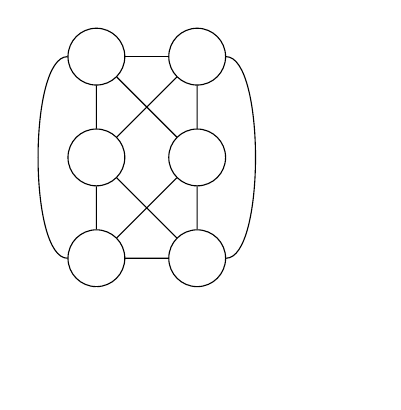
\begin{tikzpicture}[node distance={16mm}, scale=0.8, every node/.style={scale=0.8}]
            \tikzstyle{vertex} = [circle, draw=black, text=white]
            \tikzstyle{edge} = []
            
            \node[vertex] (g1) at (0,0) {$f_{1_1}$};
            \node[vertex] (g2) [right of = g1] {$f_{1_2}$};
            \node[vertex] (g3) [below of = g1] {$f_{1_3}$};
            \node[vertex] (g4) [right of = g3] {$f_{1_4}$};
            \node[vertex] (g5) [below of = g3] {$f_{1_5}$};
            \node[vertex] (g6) [right of = g5] {$f_{1_6}$};
            \draw[edge] (g1)--(g2);
            \draw[edge] (g5)--(g6);
            \draw[edge] (g1)--(g3);
            \draw[edge] (g3)--(g5);
            \draw[edge] (g2)--(g4);
            \draw[edge] (g4)--(g6);
            \draw[edge] (g3)--(g2);
            \draw[edge] (g3)--(g6);
            \draw[edge] (g4)--(g1);
            \draw[edge] (g4)--(g5);
            \draw[edge] (g1) to [out=180,in=180,looseness=0.5] (g5);
            \draw[edge] (g2) to [out=0,in=0,looseness=0.5] (g6);
            % dummy to ensure the same height as the other subfig
            \node (l) [right of = g4] {};
            \draw[color=white] (l) to [out=315,in=270] (g5);
        \end{tikzpicture}
        \caption{
            ~A $4$-regular ($r = 4$) graph $G$ with $n=6$ vertices,
            playing a role of the input graph for the $k$-\textsc{Clique} problem and
            the starting point of our construction.
        }
    \end{subfigure}%
    ~~~~
    % H
    \begin{subfigure}[t]{.46\textwidth}
        \centering
        \begin{tikzpicture}[node distance={16mm}, scale=0.8, every node/.style={scale=0.8}]
            \tikzstyle{followerG} = [circle, draw=black]
            \tikzstyle{edgeG} = [dashed, draw=green!40, thick]
        
            \tikzstyle{edgeCompl} = []

            \tikzstyle{followerF2} = [circle, fill=red!50]
            \tikzstyle{edgeF2} = [draw=red!50]

            \tikzstyle{square} = [regular polygon, regular polygon sides=4]
            \tikzstyle{leader} = [square, fill=blue!50, label={[text=blue!50]above:$\ell$}]
            \tikzstyle{edgel} = [color=blue!50]

            % G in H
            \node[followerG] (g1) at (0,0) {$f_{1_1}$};
            \node[followerG] (g2) [right of = g1] {$f_{1_2}$};
            \node[followerG] (g3) [below of = g1] {$f_{1_3}$};
            \node[followerG] (g4) [right of = g3] {$f_{1_4}$};
            \node[followerG] (g5) [below of = g3] {$f_{1_5}$};
            \node[followerG] (g6) [right of = g5] {$f_{1_6}$};
            \draw[edgeG] (g1)--(g2);
            \draw[edgeG] (g5)--(g6);
            \draw[edgeG] (g1)--(g3);
            \draw[edgeG] (g3)--(g5);
            \draw[edgeG] (g2)--(g4);
            \draw[edgeG] (g4)--(g6);
            \draw[edgeG] (g3)--(g2);
            \draw[edgeG] (g3)--(g6);
            \draw[edgeG] (g4)--(g1);
            \draw[edgeG] (g4)--(g5);
            \draw[edgeG] (g1) to [out=180,in=180,looseness=0.5] (g5);
            \draw[edgeG] (g2) to [out=0,in=0,looseness=0.5] (g6);
            % complement
            \draw[edgeCompl] (g1)--(g6);
            \draw[edgeCompl] (g2)--(g5);
            \draw[edgeCompl] (g3)--(g4);
            % leader
            \node[leader] (l) [right of = g4] {};
            \draw[edgel] (l)--(g4);
            \draw[edgel] (l)--(g6);
            \draw[edgel] (l) to [out=45,in=90] (g1);
            \draw[edgel] (l) to [out=315,in=270] (g5);
            % partners
            \node[followerF2, label={[text=red!50]above:$f_{2_1}$}] (f2) [above of = g2] {};
            \node[followerF2, label={[text=red!50]above:$f_{2_2}$}] (f3) [left of = g3] {};
            \draw[edgeF2] (f2)--(g2);
            \draw[edgeF2] (f3)--(g3);
        \end{tikzpicture}
        \caption{
            ~A $2$-regular graph $H$ constructed from graph $G$.
            The black vertices are followers from $F_1$,
            the red vertices are followers from $F_2$ and
            the blue vertex is leader.
            The green, dashed lines represent edges from $G$, which are not present in $H$,
            but from which a potential solution $W$ of \HLshort would be picked.
        }
    \end{subfigure}
    \caption{A sample construction of graph $H$ as presented in proof \ref{proofDB}.}
    \label{fig:proofDB}
\end{figure}

% Corollaries
Because we have just shown that the \HL problem parameterized by $b+d$ is W[1]-hard even for a constant number of leaders,
we can see this straightforward corollary.
\begin{corollary}
    \HL is W[1]-hard with respect to parameters
    $|L|+b+d$, $|L|+b$, $|L|+d$, $b+b$, $|L|$, $b$ and $d$.
\end{corollary}
From which we directly get another corollary.
\begin{corollary}
    \HL is para-NP-hard with respect to $|L|$.
\end{corollary}
